\documentclass[tikz,border=10pt]{standalone}
\usepackage[scaled=0.95]{helvet}
\renewcommand{\familydefault}{\sfdefault}
\usepackage[europeanresistors,americanvoltages]{circuitikz}
\definecolor{TEJNavy}{HTML}{14213D}
\definecolor{TEJBlue}{HTML}{1769AA}
\definecolor{TEJGreen}{HTML}{147D55}
\definecolor{TEJRed}{HTML}{B42318}
\definecolor{TEJGrey}{HTML}{E9EEF5}
\begin{document}
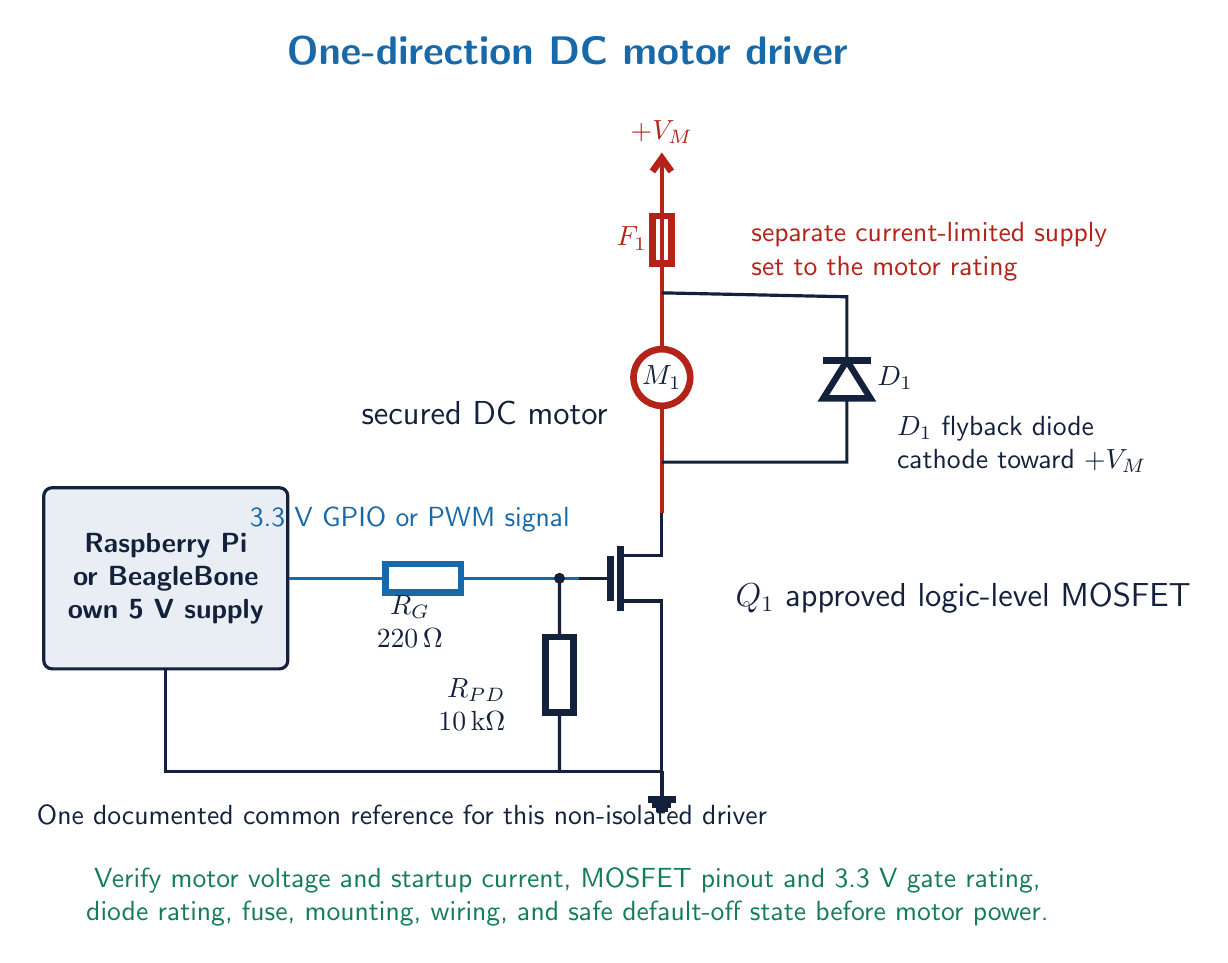
\begin{tikzpicture}[line width=1.15pt,draw=TEJNavy,text=TEJNavy,font=\sffamily]
  \ctikzset{bipoles/length=1.2cm}
  \node[font=\bfseries\Large,text=TEJBlue] at (6.8,10.0)
    {One-direction DC motor driver};

  \node[draw,rounded corners=3pt,fill=TEJGrey,minimum width=3.1cm,minimum height=2.3cm,
    align=center,font=\bfseries] (computer) at (1.7,3.3)
    {Raspberry Pi\\or BeagleBone\\own 5 V supply};

  \node[nmos,scale=1.25] (Q1) at (8.0,3.3) {};
  \node[anchor=west,font=\large] at (8.8,3.05) {$Q_1$ approved logic-level MOSFET};
  \coordinate (common) at (8.0,0.85);
  \draw (Q1.S) -- (Q1.S |- common);

  \draw[TEJBlue,very thick] (computer.east) -- ++(0.8,0)
    to[R] ++(1.8,0) -- (Q1.G);
  \draw (Q1.G) ++(-0.25,0) node[circ] (gate) {};
  \draw (gate) to[R] (gate |- common);
  \node[TEJBlue,anchor=south] at (4.8,3.75) {3.3 V GPIO or PWM signal};
  \node[TEJNavy,align=center] at (4.8,2.75) {$R_G$\\$220\,\Omega$};
  \node[TEJNavy,anchor=east,align=right] at (6.15,1.7) {$R_{PD}$\\$10\,\mathrm{k}\Omega$};

  \draw[TEJRed,very thick] (Q1.D) -- ++(0,0.65) coordinate (sw)
    to[rmeter,t={$M_1$}] ++(0,2.15) coordinate (motorTop)
    to[fuse,l={$F_1$}] ++(0,1.35)
    node[vcc] {$+V_M$};
  \node[anchor=east,font=\large] at (7.45,5.4) {secured DC motor};
  \node[TEJRed,anchor=west,align=left] at (9.0,7.45)
    {separate current-limited supply\\set to the motor rating};

  \draw (sw) -- ++(2.35,0)
    to[D,l_={$D_1$}] ++(0,2.1)
    -- (motorTop);
  \node[anchor=west,align=left] at (10.85,5.0)
    {$D_1$ flyback diode\\cathode toward $+V_M$};

  \draw[TEJNavy,very thick] (computer.south) -- (computer.south |- common) -- (common) node[ground] {};
  \node[anchor=north,align=center] at (4.7,0.55)
    {One documented common reference for this non-isolated driver};

  \node[TEJGreen,align=center] at (6.8,-0.75)
    {Verify motor voltage and startup current, MOSFET pinout and 3.3 V gate rating,\\diode rating, fuse, mounting, wiring, and safe default-off state before motor power.};
\end{tikzpicture}
\end{document}
